%%%%%%%%%%%%%%%%%%% 
% ENTAILMENT
%%%%%%%%%%%%%%%%%%%
\begin{frame}{KBP is already ``entailment''}
\w{Chris, a tenured professor at Stanford, is friends with Fei-Fei} \\
  \hspace{2em}$\Rightarrow$ \w{Chris is a tenured professor at Stanford} \\
  \hspace{2em}$\Rightarrow$ \w{Chris is a professor at Stanford} \\
  \hspace{2em}$\Rightarrow$ \w{Chris is employed by Stanford} \\
  \hspace{2em}$\Rightarrow$ (\w{Chris}; \w{employee\_of}; \w{Stanford})
\pause
\vspace{2em}

\w{Born in a small town, she took the midnight train going anywhere} \\
  \hspace{2em}$\Rightarrow$ \w{She took the midnight train going anywhere} \\
  \hspace{2em}$\Rightarrow$ \w{She took the midnight train} \\
  \hspace{2em}$\Rightarrow$ \w{She took midnight train} \\
  \hspace{2em}$\Rightarrow$ (\w{She}; \w{took}; \w{midnight train})

%\hh{Step 1:} Split sentence into clauses
%\begin{itemize}
%  \item[] \w{Chris is a tenured professor at Stanford}
%  \item[] \w{Chris, a tenured professor at Stanford, is friends with Fei-Fei}
%\end{itemize}
%\pause
%
%\hh{Sometimes challenging:}
%\begin{center}
%  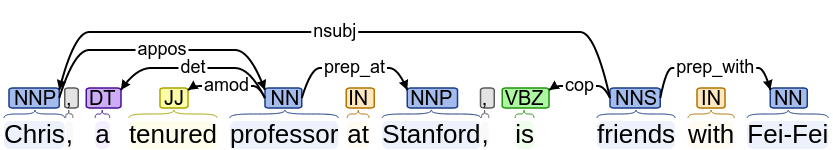
\includegraphics[scale=0.33]{../img/tree-chris-feifei.png}
%\end{center}
%
%\hh{Approach:} Train classifier for whether a dependency arc is a clause.
\end{frame}




%%%%%%%%%%%%%%%%%%% 
% TREAT AS ENTAILMENT 1
%%%%%%%%%%%%%%%%%%%
\begin{frame}{Treat As Entailment}
\begin{center}
  % Full tree
  \begin{dependency}[text only label, label style={above}]
    \begin{deptext}[column sep=-0.00cm]
      Born \& in \& a \& small \& town \&[-1ex] , \& she \& took \& the \&
        midnight \& train \& going \& anywhere \&[-1ex] . \\
    \end{deptext}
    \depedge[edge unit distance=1.25ex]{1}{5}{prep\_in}
    \depedge[edge unit distance=1.0ex]{5}{4}{amod}
    \depedge[edge unit distance=1.4ex]{5}{3}{det}
    \depedge[edge unit distance=1.0ex]{8}{1}{\textcolor<4->{darkred}{vmod}}
    \depedge[edge unit distance=2.0ex]{8}{7}{\textcolor<4->{darkblue}{nsubj}}
    \depedge[edge unit distance=1.75ex]{8}{11}{dobj}
    \depedge[edge unit distance=1.0ex]{11}{10}{nn}
    \depedge[edge unit distance=1.4ex]{11}{9}{det}
    \depedge[edge unit distance=1.0ex]{11}{12}{vmod}
    \depedge[edge unit distance=1.0ex]{12}{13}{dobj}
  \end{dependency}
  \\
  \textbf{\small{(input)}} \\
  \pause
  % arrows
  $\downarrow$ \\
  % entailments
  \begin{tabular}{ll}
    \ww{\small{she took the midnight train going anywhere}} & \ww{\small{she took the midnight train}} \\
    \ww{\small{Born in a small town, she took the midnight train}} & \ww{\small{\textbf{she took midnight train}}}  \\
    \ww{\small{Born in a town, she took the midnight train}} & $\dots$ \\
  \end{tabular}
  \pause
  \\
  % arrows 2
  $\downarrow$ \\
  % extractions
  \begin{tabular}{ll}
    (she; took; midnight train) \\
  \end{tabular}
\end{center}
\end{frame}



%%%%%%%%%%%%%%%%%%% 
% TREAT AS ENTAILMENT 2
%%%%%%%%%%%%%%%%%%%
\begin{frame}{Treat As Entailment}
\begin{center}
  % Just Clause
  \begin{dependency}[text only label, label style={above}]
    \begin{deptext}[column sep=-0.05cm]
      she \& Born \& in \& a \& small \& town \\
    \end{deptext}
    \depedge[edge unit distance=1.25ex]{2}{6}{prep\_in}
    \depedge[edge unit distance=1.0ex]{6}{5}{amod}
    \depedge[edge unit distance=1.4ex]{6}{4}{det}
    \depedge[edge unit distance=2.0ex, edge style={blue!60!black,thick}]{2}{1}{\darkblue{nsubj}}
  \end{dependency}

  \textbf{\small{(extracted clause)}} \\
  $\downarrow$ \\
  
  \begin{tabular}{l}
    \ww{\small{\textbf{she Born in small town}}} \\
    \ww{\small{she Born in a town}} \\
    \ww{\small{\textbf{she Born in town}}} \\
  \end{tabular}
  
  $\downarrow$ \\
  
  \begin{tabular}{l}
    (she; born in; small town) \\
    (she; born in; town)
  \end{tabular} 
\end{center}
\end{frame}


%%%%%%%%%%%%%%%%%%% 
% APPROACH
%%%%%%%%%%%%%%%%%%%
\begin{frame}{OpenIE Summary}
\w{Chris, a tenured professor at Stanford, is friends with Fei-Fei} \\
  \hspace{2em}$\Rightarrow$ (\w{Chris}; \w{is friends with}; \w{Fei-Fei})
\vspace{2em}

\begin{enumerate}
  \item Split a long sentence into short entailed sentences. \\
        (e.g., \w{Chris is a tenured professor at Stanford})
  \vspace{1em}
  \pause

  \item Shorten each clause maximally\\
        \checkmark \hspace{1em} \w{Chris is friends with Fei-Fei} \\
        \checkmark \hspace{1em} \w{Chris is professor} \\
        \xmark \hspace{1em} \w{Chris is friends}
  \vspace{1em}
  \pause
  
  \item Optionally segment into triples \\
\end{enumerate}
\end{frame}


%%%%%%%%%%%%%%%%%%% 
% OpenIE Results
%%%%%%%%%%%%%%%%%%%
\begin{frame}{State-of-the-art OpenIE}

KBP 2013 end-to-end evaluation:

\begin{center}
\begin{tabular}{l|cc:c}
\textbf{System} & \textbf{P} & \textbf{R} & \textbf{F$_1$} \\
\hline
UW Official            & \textbf{69.8} & 11.4   & 19.6 \\
\hline
Ollie                  & 57.4 & 4.8             & 8.9  \\
NaturalLI $-$ Nominals & 66.7 & 7.7             & 13.8 \\
\hline
Ollie + Nominal Rels   & 56.8 & 12.1            & 19.9 \\
NaturalLI              & 60.3 & \textbf{14.3}   & \textbf{23.1} \\
\end{tabular}
\end{center}
\pause
\vspace{2em}

\begin{itemize}
  \item If we add alternate names and websites: 28.6 F$_1$
  \item Context: NYU \textit{trained on KBP}: 27.7 F$_1$
  \pause
  \item MIML-RE: 36.2 F$_1$; Top system: 40.2 F$_1$
\end{itemize}
\end{frame}
